%%%%%%%%%%%%%%%%%%%%%%%%%%%%%%%%%%%%%%%%%%%%%%%%%%%%%%%%%%%%%%%%%%%
%%% Documento LaTeX 																						%%%
%%%%%%%%%%%%%%%%%%%%%%%%%%%%%%%%%%%%%%%%%%%%%%%%%%%%%%%%%%%%%%%%%%%
% Título:		Capítulo 3
% Autor:  	Ignacio Moreno Doblas
% Fecha:  	2014-02-01, actualizado 2019-11-11
% Versión:	0.5.0
%%%%%%%%%%%%%%%%%%%%%%%%%%%%%%%%%%%%%%%%%%%%%%%%%%%%%%%%%%%%%%%%%%%
% !TEX root = A0.MiTFG.tex

\chapterbegin{Fundamentos teóricos}
\label{chp:App}
\minitoc

\section{Introducción a los esquemas de señalización}
%Hablar sobre qué són los esquemas de señalización y cual es su función principal. comentar
%los esquemas (alternos,cancelación,4ppm,4ippm y pwm) y por qué se han elegido o descartado.
%Decir que no son los esquemas del estándar y que se han elegido para investigar sus ventajas e inconvenientes. 

En el ámbito de la comunicación existen múltiples esquemas de codificación digital con diferentes propiedades como 
probabilidad de bit, ciclo de trabajo, ancho de banda, etc. A la hora de estudiar un esquema de codificación para hacer 
su elección hay que tener en cuenta tres aspectos fundamentales, que son:
\begin{itemize}
    \item Flickering: se define como el cambio de la luz provocado por la conmutación entre encendido 
y apagado (1 y 0) en intervalos muy cortos. 
Estos parpadeos, si se producen a una velocidad perceptible por el ojo humano, pueden llegar a ser molestos y causar dolor. 
    \item Rendimiento óptico.
    \item La capacidad para controlar la atenuación o el dimming, provocado por por la variación de la intensidad de la luz, 
    en esquemas de codificación con ancho de pulso de la señal variable. 
\end{itemize} 

El estándar de comunicaciones por luz visible IEEE 802.15.7 usa como esquema de señalización la codificación Manchester. 
Continuando con el estudio de los esquemas de señalización,
a continuación, se van a desarrollar otras opciones de esquemas de codificación con características diferentes
para estudiar su eficacia e impacto en las comunicaciones por luz visible.
Los esquemas a desarrollar son codificación por pulsos alternos, cancelación de pulsos y 4-ppm. También se hará una 
comparativa de 4-ppm frente a Inverse 4-ppm para comparar sus prestaciones y el efecto de transmitir mayor cantidad 
de ``unos'' que de ``ceros''.

Es importante destacar que en un primer momento también se planteó el desarrollo de codificación 4-PWM pero se descartó su 
implementación debido a su escasa capacidad para controlar el dimming. Esto provocaba que la intensidad de la luz 
fluctuara mucho a lo largo de una transmisión siendo perceptible y molesto para el ojo humano.

\section{Pulsos alternos}
Comentar teóricamente en que consiste este esquema (miller pero con una opción menos y alternando).
Y que apenas está implementado y desarrollado en ningún sitio.

Dibujar y comentar el diagrama de trellis de este esquema para la codificación/decodificación de la señal.
\vspace{2cm}

\begin{figure}[ht]
    \centering
    %   TRELLIS PULSOS ALTERNOS

\tikzstyle{state}=[shape=circle,draw=blue!50,fill=blue!20,inner sep=2pt]
\def\desp{1.5}%
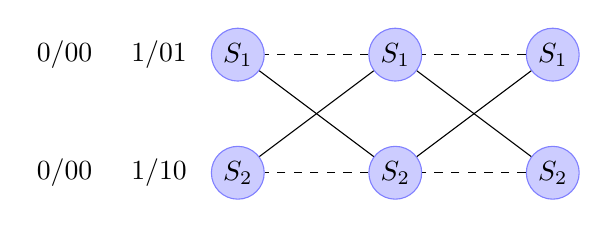
\begin{tikzpicture}[]
% 1st column
\draw (0,\desp) node[name=s1_1,state] {$S_1$} node[xshift=-2.2cm]{$0/00$}node[xshift=-1cm]{$1/01$};
\draw (0,0) node[name=s2_1,state] {$S_2$} node[xshift=-2.2cm]{$0/00$}node[xshift=-1cm]{$1/10$};
% 2nd column

\node[state] (s1_2) at (2,\desp) {$S_1$}
    edge[dashed] (s1_1)
    edge[thin] (s2_1);
\node[state] (s2_2) at (2,0) {$S_2$}
    edge[thin] (s1_1)
    edge[dashed] (s2_1);

% 3rd column

\node[state] (s1_3) at (4,\desp) {$S_1$}
    edge[dashed] (s1_2)
    edge[thin] (s2_2);
\node[state] (s2_3) at (4,0) {$S_2$}
    edge[thin] (s1_2)
    edge[dashed] (s2_2);
\end{tikzpicture}

\hspace{1cm}--------- $1$ ---------

\hspace{1cm} - - - - - $0$ - - - - -

    \caption{\small{Diagrama de Trellis de la codificación pulsos alternos.}}
    \label{trellis_alternos}%
\end{figure}

si encuentro algo hablar sobre cual es su espectro y las diferencias respecto a los del estándar

Desarrollar por qué es un esquema no equiprobable haciendo los cálculos correspondientes.

Comentar si se encuentra la ber y sus prestaciones

\section{Pulsos alternos con cancelación de pulsos}
Comentar teóricamente en que consiste este esquema (alternos pero eliminando pulsos).
Y que apenas está implementado y desarrollado en ningún sitio.

Dibujar y comentar el diagrama de trellis de este esquema para la codificación/decodificación de la señal.

\begin{figure}[ht]
    \centering
    %CANCELACION
\tikzstyle{state}=[shape=circle,draw=blue!50,fill=blue!20,inner sep=2pt]
\def\desp{1.5}%
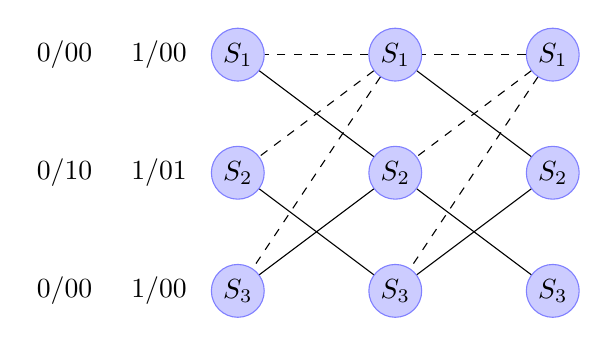
\begin{tikzpicture}[]
% 1st column
\draw (0,3*\desp) node[name=s1_1,state] {$S_1$} node[xshift=-2.2cm]{$0/00$}node[xshift=-1cm]{$1/00$};
\draw (0,2*\desp) node[name=s2_1,state] {$S_2$} node[xshift=-2.2cm]{$0/10$}node[xshift=-1cm]{$1/01$};
\draw (0,\desp) node[name=s3_1,state] {$S_3$} node[xshift=-2.2cm]{$0/00$}node[xshift=-1cm]{$1/00$};

% 2nd column

\node[state] (s1_2) at (2,3*\desp) {$S_1$}
    edge[dashed] (s1_1)
    edge[dashed] (s2_1)
    edge[dashed] (s3_1);
\node[state] (s2_2) at (2,2*\desp) {$S_2$}
    edge[thin] (s1_1)
    edge[thin] (s3_1);
\node[state] (s3_2) at (2,\desp) {$S_3$}
    edge[thin] (s2_1);

% 3d column

\node[state] (s1_3) at (4,3*\desp) {$S_1$}
    edge[dashed] (s1_2)
    edge[dashed] (s2_2)
    edge[dashed] (s3_2);
\node[state] (s2_3) at (4,2*\desp) {$S_2$}
    edge[thin] (s1_2)
    edge[thin] (s3_2);
\node[state] (s3_3) at (4,\desp) {$S_3$}
    edge[thin] (s2_2);


\end{tikzpicture}

\hspace{1cm}--------- $1$ ---------

\hspace{1cm}- - - - - $0$ - - - - -
%\line(1,0){2cm}  $1$ \line(1,0){2cm}


% 1 linea continua, 0 linea discontinua
    \caption{\small{Diagrama de Trellis de la codificación cancelación de pulsos.}}
    \label{trellis_cancelacion}%
\end{figure}

si encuentro algo hablar sobre cual es su espectro y las diferencias respecto a los del estándar

Desarrollar por qué es un esquema no equiprobable haciendo los cálculos correspondientes.

Comentar si se encuentra la ber y sus prestaciones

\section{4-PPM}
Explayarme mucho más porque hay mucha más información.
Comentar teóricamente en que consiste este esquema.
Y que apenas está implementado y desarrollado en ningún sitio.

Dibujar y comentar el diagrama de trellis de este esquema para la codificación/decodificación de la señal.

si encuentro algo hablar sobre cual es su espectro y las diferencias respecto a los del estándar

Desarrollar por qué es un esquema no equiprobable haciendo los cálculos correspondientes.

Comentar si se encuentra la ber y sus prestaciones

\section{Comparativa 4-PPM frente a Inverse 4-PPM}
Comparar estos dos esquemas y comentar ventajas e inconvenientes.
%https://ieeexplore.ieee.org/stamp/stamp.jsp?tp=&arnumber=6614862
%https://ieeexplore.ieee.org/stamp/stamp.jsp?tp=&arnumber=567560&tag=1

\section{Sistemas de decisión}
%Hablar sobre las técnicas usadas --> hard-decoding, soft-decoding y algoritmo de Viterbi
%Tener en cuenta el mapeo que se realiza para poner la señal en el rango [-8192,8191]
En este apartado se van a describir los diferentes sistemas de decisión para interpretar la señal recibida de la mejor 
manera posible que se han implementado. Para ello, se van a desarrollar 
sus características más representativas así como sus ventajas e inconvenientes.

\subsection{Hard-decoding}


\subsection{Soft-decoding}
aaaaaaaaaa
aaaaaaaaaa

aaaaaaaa
\subsection{Algoritmo de Viterbi}

% \begin{figure}[htbp]
%     \centering
%     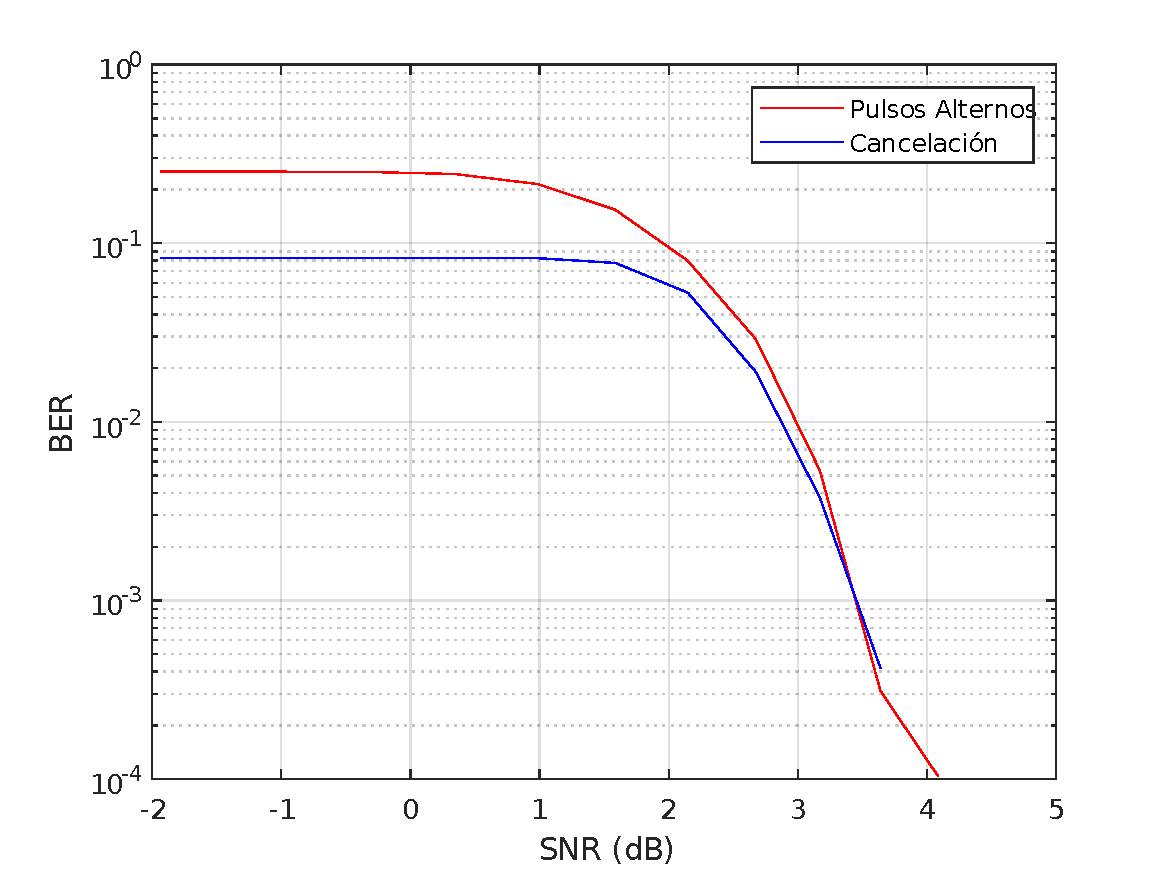
\includegraphics[scale=0.75]{./figuras/Viterbi_pulsos_cancelacion.pdf}
%     \caption{\small{Viterbi.}}
%     \label{Viterbi}%
% \end{figure}

\subsection{Comparativa entre los sistemas de decisión}
A continuación, se va a comparar la tasa de error de bit (BER) de los distintos esquemas de decisión, para cada esquema 
de codificación, en función de la relación señal a ruido (SNR), que varia con la distancia (disminuyendo la 
amplitud de la señal), para verificar la mejora que se produce entre cada sistema de decisión.

Para pulsos alternos, la principal mejora se nota con la aplicación del algoritmo de Viterbi.

Para cancelación de pulsos la aplicación del algoritmo de Viterbi es muy importante ya que, como se comentó anteriormente,
se descartan muchas opciones al mirar un pasado.

Para 4ppm el uso de soft-decoding implica una gran mejora debido a la posibilidad de buscar el bit mayor ya que solo 
se recibe un '1' por cuarteto de bits.

%%FOTOS DE ALTERNOS (HARD,SOFT,VITERBI), CANCELACION (HARD,SOFT,VITERBI) Y 4PPM(HARD,SOFT)

%%%%%%%% NO SE SI PONER UN APARTADO DE COMPARATIVA ENTRE CODIFICACIONES SEGUN EL SISTEMA DE DECISION O PONER LAS FOTOS
%%% DENTRO DE CADA ESQUEMA %%%%%%%%%%%%%%%%%%%%%%%%%%


\chapterend{}
